% Options for packages loaded elsewhere
% Options for packages loaded elsewhere
\PassOptionsToPackage{unicode}{hyperref}
\PassOptionsToPackage{hyphens}{url}
\PassOptionsToPackage{dvipsnames,svgnames,x11names}{xcolor}
%
\documentclass[
  conference,
  letterpaper]{IEEEtran}
\usepackage{xcolor}
\usepackage{amsmath,amssymb}
\setcounter{secnumdepth}{-\maxdimen} % remove section numbering
\usepackage{iftex}
\ifPDFTeX
  \usepackage[T1]{fontenc}
  \usepackage[utf8]{inputenc}
  \usepackage{textcomp} % provide euro and other symbols
\else % if luatex or xetex
  \usepackage{unicode-math} % this also loads fontspec
  \defaultfontfeatures{Scale=MatchLowercase}
  \defaultfontfeatures[\rmfamily]{Ligatures=TeX,Scale=1}
\fi
\usepackage{lmodern}
\ifPDFTeX\else
  % xetex/luatex font selection
\fi
% Use upquote if available, for straight quotes in verbatim environments
\IfFileExists{upquote.sty}{\usepackage{upquote}}{}
\IfFileExists{microtype.sty}{% use microtype if available
  \usepackage[]{microtype}
  \UseMicrotypeSet[protrusion]{basicmath} % disable protrusion for tt fonts
}{}
\makeatletter
\@ifundefined{KOMAClassName}{% if non-KOMA class
  \IfFileExists{parskip.sty}{%
    \usepackage{parskip}
  }{% else
    \setlength{\parindent}{0pt}
    \setlength{\parskip}{6pt plus 2pt minus 1pt}}
}{% if KOMA class
  \KOMAoptions{parskip=half}}
\makeatother
% Make \paragraph and \subparagraph free-standing
\makeatletter
\ifx\paragraph\undefined\else
  \let\oldparagraph\paragraph
  \renewcommand{\paragraph}{
    \@ifstar
      \xxxParagraphStar
      \xxxParagraphNoStar
  }
  \newcommand{\xxxParagraphStar}[1]{\oldparagraph*{#1}\mbox{}}
  \newcommand{\xxxParagraphNoStar}[1]{\oldparagraph{#1}\mbox{}}
\fi
\ifx\subparagraph\undefined\else
  \let\oldsubparagraph\subparagraph
  \renewcommand{\subparagraph}{
    \@ifstar
      \xxxSubParagraphStar
      \xxxSubParagraphNoStar
  }
  \newcommand{\xxxSubParagraphStar}[1]{\oldsubparagraph*{#1}\mbox{}}
  \newcommand{\xxxSubParagraphNoStar}[1]{\oldsubparagraph{#1}\mbox{}}
\fi
\makeatother


\usepackage{longtable,booktabs,array}
\usepackage{calc} % for calculating minipage widths
% Correct order of tables after \paragraph or \subparagraph
\usepackage{etoolbox}
\makeatletter
\patchcmd\longtable{\par}{\if@noskipsec\mbox{}\fi\par}{}{}
\makeatother
% Allow footnotes in longtable head/foot
\IfFileExists{footnotehyper.sty}{\usepackage{footnotehyper}}{\usepackage{footnote}}
\makesavenoteenv{longtable}
\usepackage{graphicx}
\makeatletter
\newsavebox\pandoc@box
\newcommand*\pandocbounded[1]{% scales image to fit in text height/width
  \sbox\pandoc@box{#1}%
  \Gscale@div\@tempa{\textheight}{\dimexpr\ht\pandoc@box+\dp\pandoc@box\relax}%
  \Gscale@div\@tempb{\linewidth}{\wd\pandoc@box}%
  \ifdim\@tempb\p@<\@tempa\p@\let\@tempa\@tempb\fi% select the smaller of both
  \ifdim\@tempa\p@<\p@\scalebox{\@tempa}{\usebox\pandoc@box}%
  \else\usebox{\pandoc@box}%
  \fi%
}
% Set default figure placement to htbp
\def\fps@figure{htbp}
\makeatother


% definitions for citeproc citations
\NewDocumentCommand\citeproctext{}{}
\NewDocumentCommand\citeproc{mm}{%
  \begingroup\def\citeproctext{#2}\cite{#1}\endgroup}
\makeatletter
 % allow citations to break across lines
 \let\@cite@ofmt\@firstofone
 % avoid brackets around text for \cite:
 \def\@biblabel#1{}
 \def\@cite#1#2{{#1\if@tempswa , #2\fi}}
\makeatother
\newlength{\cslhangindent}
\setlength{\cslhangindent}{1.5em}
\newlength{\csllabelwidth}
\setlength{\csllabelwidth}{3em}
\newenvironment{CSLReferences}[2] % #1 hanging-indent, #2 entry-spacing
 {\begin{list}{}{%
  \setlength{\itemindent}{0pt}
  \setlength{\leftmargin}{0pt}
  \setlength{\parsep}{0pt}
  % turn on hanging indent if param 1 is 1
  \ifodd #1
   \setlength{\leftmargin}{\cslhangindent}
   \setlength{\itemindent}{-1\cslhangindent}
  \fi
  % set entry spacing
  \setlength{\itemsep}{#2\baselineskip}}}
 {\end{list}}
\usepackage{calc}
\newcommand{\CSLBlock}[1]{\hfill\break\parbox[t]{\linewidth}{\strut\ignorespaces#1\strut}}
\newcommand{\CSLLeftMargin}[1]{\parbox[t]{\csllabelwidth}{\strut#1\strut}}
\newcommand{\CSLRightInline}[1]{\parbox[t]{\linewidth - \csllabelwidth}{\strut#1\strut}}
\newcommand{\CSLIndent}[1]{\hspace{\cslhangindent}#1}



\setlength{\emergencystretch}{3em} % prevent overfull lines

\providecommand{\tightlist}{%
  \setlength{\itemsep}{0pt}\setlength{\parskip}{0pt}}



 


\usepackage{tikz}
\usetikzlibrary{arrows.meta,positioning,shapes.geometric}
\usepackage{amsmath, amssymb, amsthm}
\usepackage{booktabs}
\usepackage{graphicx}
\usepackage{float}
\usepackage{multirow}
\usepackage{algorithm}
\usepackage{algorithmic}
\usepackage{setspace}
\usepackage{caption}
\usepackage{hyperref}
\makeatletter
\@ifpackageloaded{caption}{}{\usepackage{caption}}
\AtBeginDocument{%
\ifdefined\contentsname
  \renewcommand*\contentsname{Table of contents}
\else
  \newcommand\contentsname{Table of contents}
\fi
\ifdefined\listfigurename
  \renewcommand*\listfigurename{List of Figures}
\else
  \newcommand\listfigurename{List of Figures}
\fi
\ifdefined\listtablename
  \renewcommand*\listtablename{List of Tables}
\else
  \newcommand\listtablename{List of Tables}
\fi
\ifdefined\figurename
  \renewcommand*\figurename{Figure}
\else
  \newcommand\figurename{Figure}
\fi
\ifdefined\tablename
  \renewcommand*\tablename{Table}
\else
  \newcommand\tablename{Table}
\fi
}
\@ifpackageloaded{float}{}{\usepackage{float}}
\floatstyle{ruled}
\@ifundefined{c@chapter}{\newfloat{codelisting}{h}{lop}}{\newfloat{codelisting}{h}{lop}[chapter]}
\floatname{codelisting}{Listing}
\newcommand*\listoflistings{\listof{codelisting}{List of Listings}}
\makeatother
\makeatletter
\makeatother
\makeatletter
\@ifpackageloaded{caption}{}{\usepackage{caption}}
\@ifpackageloaded{subcaption}{}{\usepackage{subcaption}}
\makeatother
\usepackage{bookmark}
\IfFileExists{xurl.sty}{\usepackage{xurl}}{} % add URL line breaks if available
\urlstyle{same}
\hypersetup{
  colorlinks=true,
  linkcolor={blue},
  filecolor={Maroon},
  citecolor={Blue},
  urlcolor={Blue},
  pdfcreator={LaTeX via pandoc}}


\author{}
\date{}
\begin{document}


\title{Sentiment Classification on GoEmotions: A Comparative Study of Text Classification Methods}
\author{
  \IEEEauthorblockN{Anuruddha Ekanayake}
  \IEEEauthorblockA{\textit{School of Computing} \\
    \textit{University of Nebraska-Lincoln}\\
    Lincoln, USA \\
    aekanayake2@nebraska.edu}
  \and
  \IEEEauthorblockN{Arian Alai}
  \IEEEauthorblockA{\textit{Institute of Agriculture and Natural Resources} \\
    \textit{University of Nebraska-Lincoln}\\
    Lincoln, USA \\
    aalai4@nebraska.edu}
  \and
  \IEEEauthorblockN{Daniel Crow}
  \IEEEauthorblockA{\textit{School of Computing} \\
    \textit{University of Nebraska-Lincoln}\\
    Lincoln, USA \\
    dcrow2@nebraska.edu}
}
\maketitle

\begin{abstract}
In this work, we study sentiment classification on the GoEmotions dataset by mapping fine-grained emotions to four coarse sentiment categories: positive, negative, neutral and ambiguous. To simplify the task in a single-label setting, only samples with exactly one emotion label are retained. We train and compare two classification models: a Term Frequency-Inverse Document Frequency (TF-IDF) feature pipeline with a Logistic Regression classifier, and a fine-tuned DistilBERT transformer. Our experimental results show that the TF-IDF + Logistic Regression baseline achieves a classification accuracy of 0.636 (95\% Confidence Interval (CI) [0.622, 0.650]) and macro-F1 of 0.601 (95\% CI [0.585, 0.616]). Fine-tuning DistilBERT on the full training dataset yields a test accuracy of 0.715 (95\% CI [0.703, 0.728]) and macro-F1 of 0.684 (95\% CI [0.669, 0.699]). Since the 95\% confidence intervals for accuracy do not overlap, we conclude that the transformer-based model provides a statistically significant improvement over the linear baseline.
\end{abstract}

\section{Introduction}\label{introduction}

Emotion and sentiment analysis are fundamental tasks in Natural Language
Processing (NLP). These tasks enable the conversion of raw, human
language into structured data denoting emotional intent, making them
useful techniques for a wide range of applications, including customer
service, social media analysis, and public opinion monitoring. The
widespread adoption of social media has especially led to a massive
influx of informal text, which is often characterized by noisy writing,
slang, and complex emotional expressions. Standard sentiment analysis
(classifying text into positive, negative, or neutral) is often
insufficient for capturing the nuances of these diverse expressions.

The GoEmotions dataset (Demszky et al. 2020) is a large, human-annotated
corpus with approximately 58,000 Reddit comments labeled with 28
fine-grained emotion categories. In this project, we address a
simplified formulation of the task: 4-way single-label sentiment
classification. We filter the comments to keep only those with exactly
one emotion label, and map that label to one of four sentiment classes:
\emph{positive}, \emph{negative}, \emph{neutral}, or \emph{ambiguous}.

To address this task, we compare two modeling approaches. The first is a
baseline model that combines TF-IDF features derived from word- and
character-level n-grams with a Logistic Regression classifier. The
second is a transformer-based approach that fine-tunes a pre-trained
DistilBERT model on the training data.

We evaluate both models on the test split, report their classification
accuracy and macro-F1 scores along with 95\% bootstrap confidence
intervals. We also analyze their per-class performance to determine the
best-performing model for the task.

\section{Problem Description}\label{problem-description}

The sentiment classification task is framed as a supervised single-label
classification problem. Given an input text string \(x \in \mathcal{X}\)
representing a single Reddit comment, the objective is to predict a
label \(y \in \mathcal{Y}\). Prior to feature extraction, the text is
preprocessed by collapsing consecutive whitespace, removing newline
characters, and stripping leading and trailing whitespace. The label
space is defined as

\[\mathcal{Y} = \{\text{negative}, \text{neutral}, \text{positive}, \text{ambiguous}\}\]

\subsection{Sentiment Mapping}\label{sentiment-mapping}

We map the original 28 GoEmotions categories to our target sentiment
classes as follows:

\begin{itemize}
\tightlist
\item
  \textbf{Positive:} admiration, amusement, approval, caring, desire,
  excitement, gratitude, joy, love, optimism, pride, relief.
\item
  \textbf{Negative:} anger, annoyance, disappointment, disapproval,
  disgust, embarrassment, fear, grief, nervousness, remorse, sadness.
\item
  \textbf{Ambiguous:} confusion, curiosity, realization, surprise.
\item
  \textbf{Neutral:} neutral.
\end{itemize}

To formulate the problem as a single-label classification task, we
retain only comments with exactly one emotion label.

\section{Methodology}\label{methodology}

We compare a linear baseline with a transformer-based model for
sentiment classification.

\subsection{TF-IDF + Logistic Regression
(Baseline)}\label{tf-idf-logistic-regression-baseline}

The baseline model maps raw comments into a sparse vector space using
term frequency-inverse document frequency (TF-IDF) feature weighting.
Character-level n-grams are extracted to capture subword details (such
as punctuation patterns and word endings), while word-level n-grams
capture explicit emotional descriptors. By considering both unigrams and
bigrams, the vectorizer captures local lexical patterns, including
frequently occurring phrases such as short negation expressions. The
resulting vectors are passed to a multi-class Logistic Regression
classifier, which models the probability of each sentiment class as a
linear combination of the lexical features. To prevent overfitting to
the large feature space, the model is trained with L2 regularization,
and class weights are adjusted to compensate for training set imbalance.

\subsection{Fine-Tuned DistilBERT
(Transformer)}\label{fine-tuned-distilbert-transformer}

DistilBERT (Sanh et al. 2019) is a compact transformer model derived
from BERT via knowledge distillation to learn deep contextualized text
representations. Unlike TF-IDF, which treats words independently of
their position, DistilBERT utilizes self-attention mechanisms to
dynamically compute representations where a word's vector changes
depending on its surrounding tokens. Input text is segmented using
WordPiece subword tokenization to mitigate out-of-vocabulary terms. The
token sequence is then processed through transformer layers to capture
long-range semantic and syntactic dependencies. For classification, the
final hidden state corresponding to the special \texttt{{[}CLS{]}} token
is used as a sequence-level representation for classification. A linear
classification layer maps this contextual vector to logits corresponding
to the target sentiment classes. During training, the pre-trained
encoder weights and the classification head are jointly fine-tuned on
our target data.

\section{Experimental Setup}\label{experimental-setup}

This section details the dataset partitions, model hyperparameters, and
metrics used in our evaluation.

\subsection{Dataset Splits}\label{dataset-splits}

After filtering multi-label comments and mapping the original 28
emotions into four sentiment categories, the resulting dataset is split
into training, validation, and test sets. The class counts for each
split are:

\begin{itemize}
\tightlist
\item
  \textbf{Train Set:} 36,308 samples (12,920 positive, 12,823 neutral,
  7,012 negative, 3,553 ambiguous).
\item
  \textbf{Validation Set:} 4,548 samples (1,668 positive, 1,592 neutral,
  853 negative, 435 ambiguous).
\item
  \textbf{Test Set:} 4,590 samples (1,606 neutral, 1,603 positive, 932
  negative, 449 ambiguous).
\end{itemize}

\subsection{Hyperparameters \& Training
Settings}\label{hyperparameters-training-settings}

For the \textbf{TF-IDF + Logistic Regression} baseline, features are
computed using word and character n-grams with \(n \in \{1,2\}\). We
restrict the vocabulary to the top 50,000 features, filter out features
appearing in only one document (\(min\_df = 2\)), and apply sublinear
term-frequency scaling (\(\text{tf} \leftarrow 1 + \log(\text{tf})\)).
The Logistic Regression classifier is regularized with an inverse
strength parameter of \(C = 1.0\) and optimized using the L-BFGS solver
with a maximum of 1,000 iterations.

For \textbf{DistilBERT}, input texts are padded or truncated to a
maximum sequence length of 64 tokens. The model is fine-tuned for two
epochs using the AdamW optimizer with a learning rate of
\(2 \times 10^{-5}\) and a batch size of 16. Training was conducted
using GPU acceleration.

\subsection{Evaluation Metrics}\label{evaluation-metrics}

We evaluate both models on the held-out test split using:

\begin{itemize}
\tightlist
\item
  \textbf{Classification Accuracy:} The percentage of comments predicted
  correctly.
\item
  \textbf{Macro-F1 Score:} The unweighted average of F1-scores across
  all sentiment classes, ensuring that minority classes (such as
  ``ambiguous'') are weighted equally.
\item
  \textbf{Per-Class F1-Score:} To evaluate performance variations across
  specific sentiments.
\end{itemize}

To quantify uncertainty, we estimate 95\% confidence intervals (CI) for
both accuracy and macro-F1 using bootstrapping with \(N = 1,000\)
resamples.

\section{Results and Discussion}\label{results-and-discussion}

\subsection{Overall Performance}\label{overall-performance}

Table 1 summarizes the overall performance of the two models on the test
set.

\begin{table}[h]
\centering
\caption{Overall test performance of the classification models.}
\small
\begin{tabular}{@{}lcc@{}}
\toprule
Model & Accuracy (95\% CI) & Macro-F1 (95\% CI) \\
\midrule
TF-IDF + LogReg & 0.636\,[0.622, 0.650] & 0.601\,[0.585, 0.616] \\
DistilBERT & \textbf{0.715}\,[0.703, 0.728] & \textbf{0.684}\,[0.669, 0.699] \\
\bottomrule
\end{tabular}
\end{table}

DistilBERT substantially outperformed the TF-IDF baseline, improving
accuracy from 0.636 to 0.715 (+7.9 percentage points) and macro-F1 from
0.601 to 0.684 (+8.3 percentage points). Furthermore, the bootstrap
confidence intervals for accuracy show a clear separation between the
two models, providing strong evidence that the observed improvement is
unlikely to be due to sampling variability.

\subsection{Per-Class F1 Analysis}\label{per-class-f1-analysis}

Table 2 reports the F1-score for each sentiment class.

\begin{table}[h]
\centering
\caption{Per-class F1-scores on the test set.}
\small
\begin{tabular}{@{}lccc@{}}
\toprule
Class & TF-IDF + LogReg & DistilBERT & $\Delta$ \\
\midrule
negative & 0.576 & \textbf{0.674} & +0.098 \\
neutral & 0.629 & \textbf{0.679} & +0.050 \\
positive & 0.747 & \textbf{0.818} & +0.071 \\
ambiguous & 0.452 & \textbf{0.566} & +0.114 \\
\bottomrule
\end{tabular}
\end{table}

DistilBERT achieved higher F1-scores for every sentiment class. The
largest improvements occurred for the \textbf{ambiguous} (+0.114) and
\textbf{negative} (+0.098) classes, suggesting that contextual
transformer representations are particularly effective for recognizing
indirect, nuanced, and context-dependent emotional expressions. More
modest gains were observed for the \textbf{positive} (+0.071) and
\textbf{neutral} (+0.050) classes, indicating that these categories are
comparatively easier for both models to identify.

\subsection{Visualizations}\label{visualizations}

The performance comparisons are illustrated in the figures below.
Fig.\ref{fig-accuracy} displays the overall test accuracy with 95\%
bootstrap confidence intervals, Fig.\ref{fig-f1-plot} compares the
per-class F1-scores, and
Figs.\ref{fig-cm-baseline}--\ref{fig-cm-distilbert} present the
normalized confusion matrices for both models.

\begin{figure}[t]
\centering
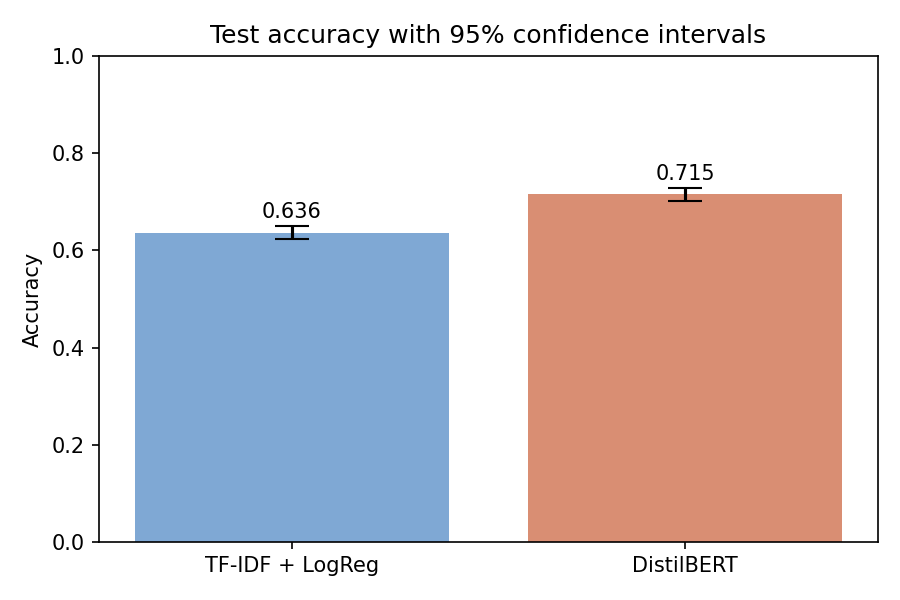
\includegraphics[width=\columnwidth]{results/accuracy_ci.png}
\caption{Classification accuracy with 95\% bootstrap confidence intervals.}
\label{fig-accuracy}
\end{figure}

\begin{figure}[t]
\centering
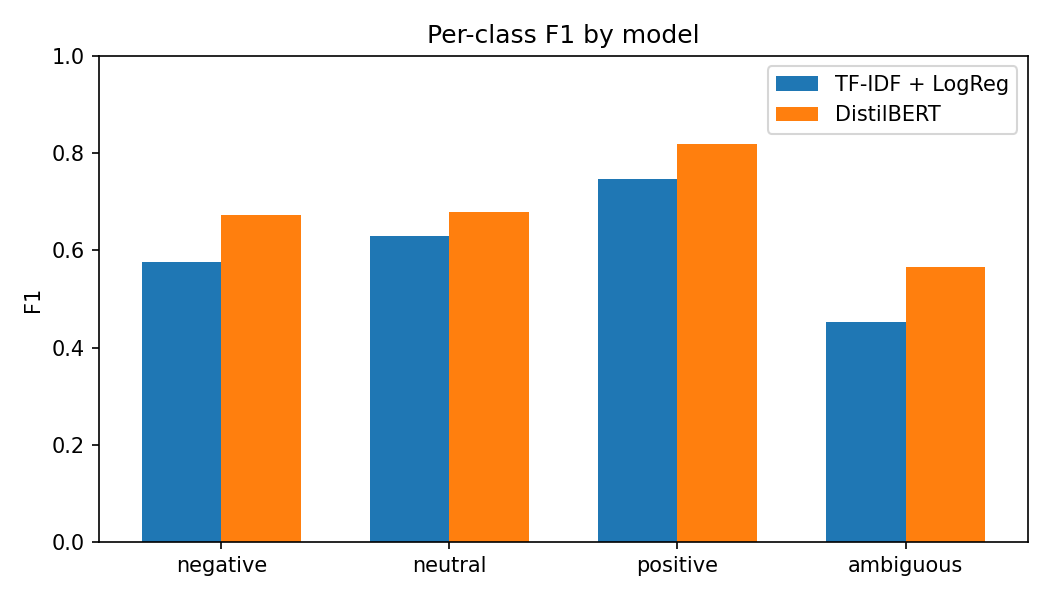
\includegraphics[width=\columnwidth]{results/per_class_f1.png}
\caption{Per-class F1-scores on the test set.}
\label{fig-f1-plot}
\end{figure}

\begin{figure}[t]
\centering
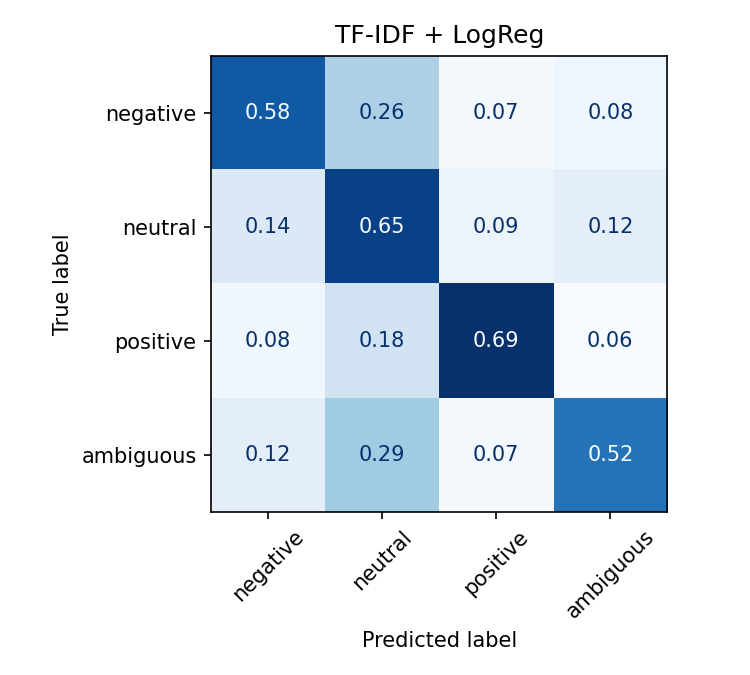
\includegraphics[width=\columnwidth]{results/cm_baseline.png}
\caption{Normalized confusion matrix for TF-IDF + Logistic Regression.}
\label{fig-cm-baseline}
\end{figure}

\begin{figure}[t]
\centering
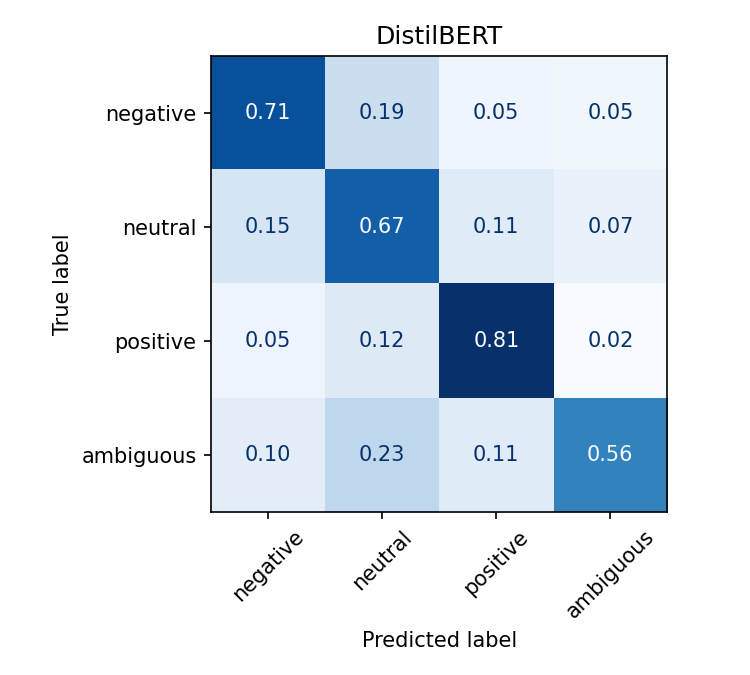
\includegraphics[width=\columnwidth]{results/cm_transformer.png}
\caption{Normalized confusion matrix for fine-tuned DistilBERT.}
\label{fig-cm-distilbert}
\end{figure}

\subsection{Error Analysis}\label{error-analysis}

To understand the limitations of both modeling approaches, we conduct an
error analysis on their classification failures on the test split.

\subsubsection{TF-IDF + Logistic Regression
Errors}\label{tf-idf-logistic-regression-errors}

\begin{itemize}
\tightlist
\item
  \textbf{Blindness to Valence Shifts and Negation:} Because the model
  relies on sparse n-gram occurrences, it is blind to contextual shifts
  in sentiment. For example, it misclassified the negative comment
  \emph{``I'm sorry to hear that friend :(. It's for the best\ldots{}''}
  as \emph{positive} due to the high coefficients of words like
  \texttt{"best"}, \texttt{"friend"}, and \texttt{"accept"}. Similarly,
  it misclassified \emph{``It's wonderful because it's awful.''} (which
  is \emph{positive}) as \emph{negative} due to the presence of the word
  \texttt{"awful"}.
\item
  \textbf{Over-reliance on Superficial Indicators:} The baseline is
  highly sensitive to explicit lexical cues. For example, features with
  large positive-class coefficients, such as \texttt{"lol"} (10.28) and
  \texttt{"thanks"} (10.18), strongly influence \emph{positive}
  predictions, even in sarcastic context. Conversely, since the
  \emph{neutral} class lacks distinct emotional words, the model is
  forced to rely on noisy structural features like \texttt{"they"}
  (2.31) or bot commands like \texttt{"remindme"} (1.55), which
  generalize poorly.
\item
  \textbf{Out-of-Vocabulary (OOV) and Spelling Variations:} The
  word-level representation cannot generalize to spelling variations,
  typos, or slang unseen during training.
\end{itemize}

\subsubsection{DistilBERT Errors}\label{distilbert-errors}

\begin{itemize}
\tightlist
\item
  \textbf{Sensitivity to Aggressive Phrasing in Neutral Comments:}
  DistilBERT tends to over-predict the \emph{negative} class when
  comments contain strong punctuation or demanding phrasing, even if the
  content itself is neutral. For example, it misclassified \emph{``You
  take that back right now! {[}NAME{]} does not deserve this.''}
  (labeled \emph{neutral} in GoEmotions) as \emph{negative}.
\item
  \textbf{Failure on Short, Elliptical Queries:} For short, elliptical
  queries, DistilBERT may struggle when structural cues dominate the
  meaning of the sentence. For instance, for the ambiguous question
  \emph{``out of everyone why AC?''}, DistilBERT predicted
  \emph{neutral}, whereas the baseline correctly identified it as
  \emph{ambiguous} by matching the key feature \texttt{"why"}.
\item
  \textbf{Interpretability Deficit:} Unlike the logistic regression
  baseline where the feature coefficients directly explain why a
  classification was made, DistilBERT's deep representations act as a
  black box, making individual failures difficult to debug or audit.
\end{itemize}

\section{Conclusion}\label{conclusion}

These findings demonstrate that contextual transformer models
substantially improve sentiment classification of noisy social media
text. While TF-IDF remains valuable when efficiency and interpretability
are priorities, DistilBERT provides a clear advantage for modeling
context-dependent emotional expressions.

\phantomsection\label{refs}
\begin{CSLReferences}{1}{0}
\bibitem[\citeproctext]{ref-demszky-etal-2020-goemotions}
Demszky, Dorottya, Dana Movshovitz-Attias, Jeongwoo Ko, Alan Cowen,
Gaurav Nemade, and Sujith Ravi. 2020. {``{G}o{E}motions: A Dataset of
Fine-Grained Emotions.''} In \emph{Proceedings of the 58th Annual
Meeting of the Association for Computational Linguistics}, 4040--54.
Online: Association for Computational Linguistics.
\url{https://doi.org/10.18653/v1/2020.acl-main.372}.

\bibitem[\citeproctext]{ref-sanh2019distilbert}
Sanh, Victor, Lysandre Debut, Julien Chaumond, and Thomas Wolf. 2019.
{``{D}istil{BERT}, a Distilled Version of {BERT}: Smaller, Faster,
Cheaper and Lighter.''} \emph{arXiv Preprint arXiv:1910.01108}.

\end{CSLReferences}




\end{document}
